\documentclass[11pt]{article}

\usepackage{apacite}
\usepackage{amsmath,amssymb}
\usepackage{graphicx}
\usepackage{color}
\usepackage{url}
\usepackage{fullpage}
\usepackage{setspace}
\usepackage{booktabs}
%\usepackage{lingmacros}
\usepackage{gb4e}
\usepackage{hyperref}
\hypersetup{colorlinks,breaklinks,
            linkcolor=cyan,urlcolor=cyan,
            anchorcolor=cyan,citecolor=cyan}


% useful commands
\definecolor{Red}{RGB}{255,0,0}
\newcommand{\red}[1]{\textcolor{Red}{#1}}
\newcommand{\jd}[1]{\textcolor{Red}{[jd: #1]}} 

\newcommand{\denote}[1]{\mbox{ $[\![ #1 ]\!]$}}
\newcommand{\subsubsubsection}[1]{{\em #1}}
\newcommand{\eref}[1]{(\ref{#1})}
\newcommand{\tableref}[1]{Table \ref{#1}}
\newcommand{\figref}[1]{Figure \ref{#1}}
\newcommand{\appref}[1]{Appendix \ref{#1}}
\newcommand{\sectionref}[1]{Section \ref{#1}}

\title{The weakness of epistemic \emph{must}: A pragmatic reasoning approach}
 
\author{{\large \bf Judith Degen (jdegen@stanford.edu), Gregory Scontras (scontras@stanford.edu),}\\ {\large \bf Andreas Trotzke (andreas.trotzke@uni-konstanz.de), Eva Wittenberg (ewittenberg@ucsd.edu)}}



\begin{document}

\maketitle

\red{INSERT}

\begin{abstract}
% OLD ABSTRACT:

%We present results from three studies exploring the interpretation of statements featuring the epistemic necessity modal \emph{must}, comparing these statements to utterances with weaker modals, or no modals at all. Our results demonstrate that \emph{must}-statements coincide with less certain belief states, such that ``It must be raining'' receives a weaker interpretation than bare ``It is raining.'' Rather than engineering weakness into the meaning of the word \emph{must}, our account derives its weakness as an M-implicature \cite{levinson2000}. Statements with \emph{must} are marked relative to bare statements, so they communicate a marked meaning, namely less certainty on the part of the speaker. A general model of rational inference in communication delivers the puzzlingly weak interpretation of \emph{must}.
	
\textbf{Keywords:} 
pragmatics; semantics; psycholinguistics; modals; discourse particles; German; English
\end{abstract}


\section{Introduction}

% OLD INTRO:

%Modals come in varying degrees of strength; the strongest are modals of necessity like \emph{must} or \emph{have to}. Under a quantificational treatment of modality, these necessity modals correspond to universal quantifiers over possible words (XXX citation). When used, they assert that in every (relevant) possible world, some proposition \emph{p} holds. In (\ref{must}), epistemic \emph{must} is used to assert that in every world compatible with the speaker's knowledge, it is raining. Given that knowledge corresponds to justified true belief (that which is known cannot be otherwise), from (\ref{must}) it necessarily follows that it is raining (i.e., it is not possible that it is not raining). There are other analyses of modals on the market (e.g., a scalar semantics for modals; \citeNP{lassiter2011}), but all of them share the intuitive understanding of necessity modals as maximally strong semantic objects. 
%
%\begin{exe}
%	\ex\label{inference} \begin{xlist}
%		\ex\label{might} It might be raining.
%		\ex\label{must} It must be raining. 
%		\ex\label{bare} It is raining.
%	\end{xlist}
%\end{exe}
%
%When compared with other modals, necessity modals do behave as strong: (\ref{must}) expresses a stronger statement about rain than (\ref{might}). However, when compared to the bare statement without a modal, \emph{must} and other epistemic necessity modals suddenly behave as weak, or so the liturgy goes.  At issue is the failed inference from (\ref{must}) to (\ref{bare}) first observed by \citeA{karttunen1972}: How could \emph{must p} not entail \emph{p}? If it is necessarily raining, then surely it is raining. It appears that talking about what is necessarily the case commits speakers to less than does talking about what is actually the case. \citeauthor{karttunen1972} and decades of semanticists that followed posit that the inference from (\ref{must}) to (\ref{bare}) fails because \emph{must p} is a weaker statement than bare \emph{p}. In other words, \emph{must} is weak. Our first task is to evaluate the relative strength of \emph{must}, an empirical investigation conspicuously absent from the discussion of this modal thus far. Having justified the strength of \emph{must} empirically, we may then set our sights on the proposals meant to account for \emph{must}'s meaning.
%
%Linguists split on the semantics of \emph{must}. The original ``\emph{must} is weak'' mantra, stemming from \citeA{karttunen1972}, has \emph{must p} not entail \emph{p}. There are two tacks to breaking this entailment. For \citeA{kratzer1991}, the entailment fails because  \emph{must p} is weaker than we might have thought. She weakens \emph{must} by having it quantify not just over knowledge states, but also over expectations given knowledge states -- expectations which are not always borne out. For \citeA{veltman1985}, the entailment fails because bare \emph{p} is stronger than we might have thought. He strengthens bare \emph{p} by allowing partial knowledge states, such that \emph{must p} may be true while we lack the knowledge to say whether \emph{p} is true or false. Either way, from \emph{must p} (e.g., ``It must be raining'') it does not follow that \emph{p} (e.g., ``It is raining'').
%
%\citeA{vonfintelgillies2010} lead the opposing charge, holding firm to the logic that \emph{must p} is strong, quantifying universally over epistemically possible worlds. In addition to this strong semantics, they also claim that \emph{must} is an evidential marker, presupposing that the speaker has no direct evidence of \emph{p}. However, the strength of \emph{must p} requires the speaker to have direct evidence of something that entails \emph{p}. Using a corpus of naturally-occurring examples from Ancestry.com, \citeauthor{lassiter2014salt} (\emph{to appear}) shows how \citeauthor{vonfintelgillies2010}'s implementation of a strong semantics for \emph{must} makes unreasonable claims about the knowledge states of speakers. \citeauthor{lassiter2014salt} proposes instead a weak probabilistic semantics: \emph{must p} entails that the probability of \emph{p} given the speaker's direct knowledge is greater than chance, and requires that the question of whether \emph{p} not be resolved by this direct knowledge. Thus, he returns to the original mantra of weakness while building evidential information into the semantics of \emph{must}.
%
%In an effort to inform this debate on the strength of \emph{must}, we first investigate what gets communicated via its use. Over the course of three experiments, we asses the speaker commitments, evidence strength, and listener understanding that accompany \emph{must} statements. Our findings qualitatively confirm \citeauthor{karttunen1972}'s original observation, and quantitatively demonstrate the relative weakness of \emph{must}. Moreover, they highlight the role of evidence strength in the computation of \emph{must}'s meaning -- an ingredient that has thus far been lacking from the proposed semantics for \emph{must}.
%
%We then use our findings to motivate a computational model of the meaning of \emph{must}, following \citeA{lassitergoodman2013} in their extension of the Bayesian Rational Speech Act framework \cite{frankgoodman2012}. Rather than engineering weakness relative to bare \emph{p} directly into the meaning of the word \emph{must}, our account derives its weakness as an M-implicature \cite{levinson2000}: \emph{must p} is marked (i.e., costly) relative to the bare form (\ref{bare}); the bare form is sufficiently strong already to convey \emph{p} (e.g., that it is raining), so listeners take the marked form to convey the marked meaning that the speaker arrived at the conclusion \emph{p} via an evidentially less certain route than if they had chosen the shorter, bare form. Our account accomplishes two things. First, it obviates the conceptual pitfalls of \citeauthor{vonfintelgillies2010}'s strong semantics, without treating \emph{must} as inherently weak: evidence strength is inferred from, rather than communicated by, the use of \emph{must}. Second, it implements a formal model of M-implicatures within the Rational Speech Act framework \cite{bergenetal2014}.
%
%%Our approach incorporates elements from both \citeA{vonfintelgillies2010} and \citeauthor{lassiter2014salt} \emph{to appear}: \emph{Must} is strong, but reasoning about its strong meaning yields a weaker interpretation.


In the following, we label English and German experiments as \emph{E.N} and \emph{G.N}, respectively.

\section{Experiment E.1: evidence strength}

In Exp.~E.1, we collected estimates of evidence strength.\footnote{This experiment can be viewed \href{https://web.stanford.edu/~justinek/modals_exp/evidence.html}{here}.} These estimates were used in the analysis of Experiments 2 and 3.

\subsection{Methods}

\subsubsection{Participants}

40 participants were recruited through Amazon's Mechanical Turk crowd-sourcing service, and were compensated for their participation.

\subsubsection{Materials and procedure}

Participants rated the probability of a state of affairs $q$ given a piece of evidence $e$ by adjusting a slider on a scale with endpoints labeled ``impossible'' and ``absolutely certain''. On each trial, participants first saw the context sentence ``Imagine that you are at home.'' Then the evidence $e$ for $q$ was shown, e.g., ``Dinner is usually ready around 6pm. You look at the clock and it is 6pm.'' Finally, participants were asked about the probability of $q$, e.g., ``How likely is it that dinner is ready?'' and adjusted the slider accordingly. There were four different $q$ that appeared in the ``How likely is it that $q$?'' frame:

\begin{exe}
	\ex it is raining
	\ex the coffee is cold
	\ex dinner is ready
	\ex the neighbor's dog is barking
\end{exe}

For each \emph{q}, each participant evaluated one of five possible pieces of evidence, resulting in four trials per participant. Trial order was randomized. 

Pieces of evidence were generated by taking a version of the top five most frequently generated explanations from a separate experiment in which $q$ was given to participants and they were asked to provide a free response explanation of how the speaker knows about $q$.\footnote{This experiment can be viewed \href{http://stanford.edu/~jdegen/68_modals_freeproduction/modals.html}{here}.} The full list of pieces of evidence for each $q$ can be found in \appref{sec:evidence}.


\subsection{Results and discussion}

We obtained between \red{XX} and \red{XX} ratings for each piece of evidence. We interpret the slider value between 0 (``impossible'') and 1 (``absolutely certain'') as a participant's estimate of the probability of $q$, given $e$, which we will also sometimes refer to as  \emph{evidence strength}. A histogram of mean evidence strengths is shown in \figref{fig:evidencestrength}.  We used these evidence strength ratings in the design and analyses of Experiments 2 and 3.

\begin{figure}
\red{insert figure of english and german data side by side}
\caption{Histogram of evidence strength ratings for English (Exp.~E.1, left) and German (Exp.~G.1, right).}
\label{fig:evidencestrength}
\end{figure}


\section{Experiment E.2: production}

Next, we evaluated speakers' intuitions in a forced production task, testing how likely they are to use a particular form to communicate their belief about $q$ when given different pieces of evidence.\footnote{This experiment can be viewed \href{http://stanford.edu/~jdegen/71_modals_forced_production/modals.html}{here}.}

\subsection{Methods}

\subsubsection{Participants}

We recruited 40 participants from Amazon's Mechanical Turk. Participants were compensated with a small payment.

\subsubsection{Materials and procedure}

Participants were presented with a piece of evidence (e.g., ``You see a person come in from outside with wet hair and wet clothes'') and were asked to choose one of four possible utterances to describe the situation to a friend. On each trial, they first saw a context sentence which varied by domain, e.g., ``Imagine that you are sitting in a room.'' Next, they were presented with a piece of evidence, e.g., ``Earlier today, you had seen dark clouds in the sky.'' Finally, each participant saw the same question: ``Given what you know, what do you say to a friend who is sitting in a windowless room down the hall?'' They then chose one of four possible utterances by checking a radio button, e.g., ``It's raining'', ``It must be raining'', ``It's probably raining'', ``It might be raining''. Across domains, each choice was between utterances of the forms shown in \eref{utterancechoices}.

\begin{exe}
	\ex\label{utterancechoices} \emph{Abstract form of utterance choices:}
	\begin{xlist}
		\ex $q$ (bare)
		\ex \emph{must q} (must)
		\ex \emph{probably q} (probably)
		\ex \emph{might q} (might)
		\end{xlist}
		\end{exe}
		
Each participant completed 12 trials, three per domain. For each participant and domain, three pieces of evidence were randomly sampled from the set of five. Trial order was randomized, as was the order of utterance options.

\subsection{Results and discussion}

Proportions of utterance choices for each piece of evidence are shown in \figref{fig:utterancesbyevidence} as a function of each piece of evidence's strength. In order to evaluate the effect of evidence strength on utterance choice, we conducted a mixed-effects model \red{looking at what exactly? multinomial regression?}. Of note are the following results: as evidence strength increases, the probability of producing the bare form increases (\red{XXX}). As evidence strength increases, the probability of producing \emph{must} \red{increases (XXX)}. As evidence strength increases, the probability of producing \emph{probably} \red{increases (XXX)}. And as evidence strength increases, the probability of producing \emph{might} \red{increases (XXX)}.

\begin{figure}
\red{insert figure of english and german data side by side -- but maybe only the second figure?}
\caption{Proportion of utterance choice for English (Exp.~E.2, left) and German (Exp.~G.2, right).}
\label{fig:utterances}
\end{figure}

\begin{figure}
\red{insert figure of english and german data side by side}
\caption{Proportion of utterance choice for English (Exp.~E.2, left) and German (Exp.~G.2, right) as a function of evidence strength.}
\label{fig:utterancesbyevidence}
\end{figure}

%Fig.~\ref{expt2} plots selection rates for the \emph{might}, \emph{must}, and \emph{bare} utterances against the evidence strength estimates from Experiment 1. Participants were more likely to choose the more marked \emph{must} form over the bare form as evidence strength decreased ($\beta$=5.4, \emph{SE}=2.4, \emph{p}$<$0.05). 
%
%\begin{figure}
%\centering
%{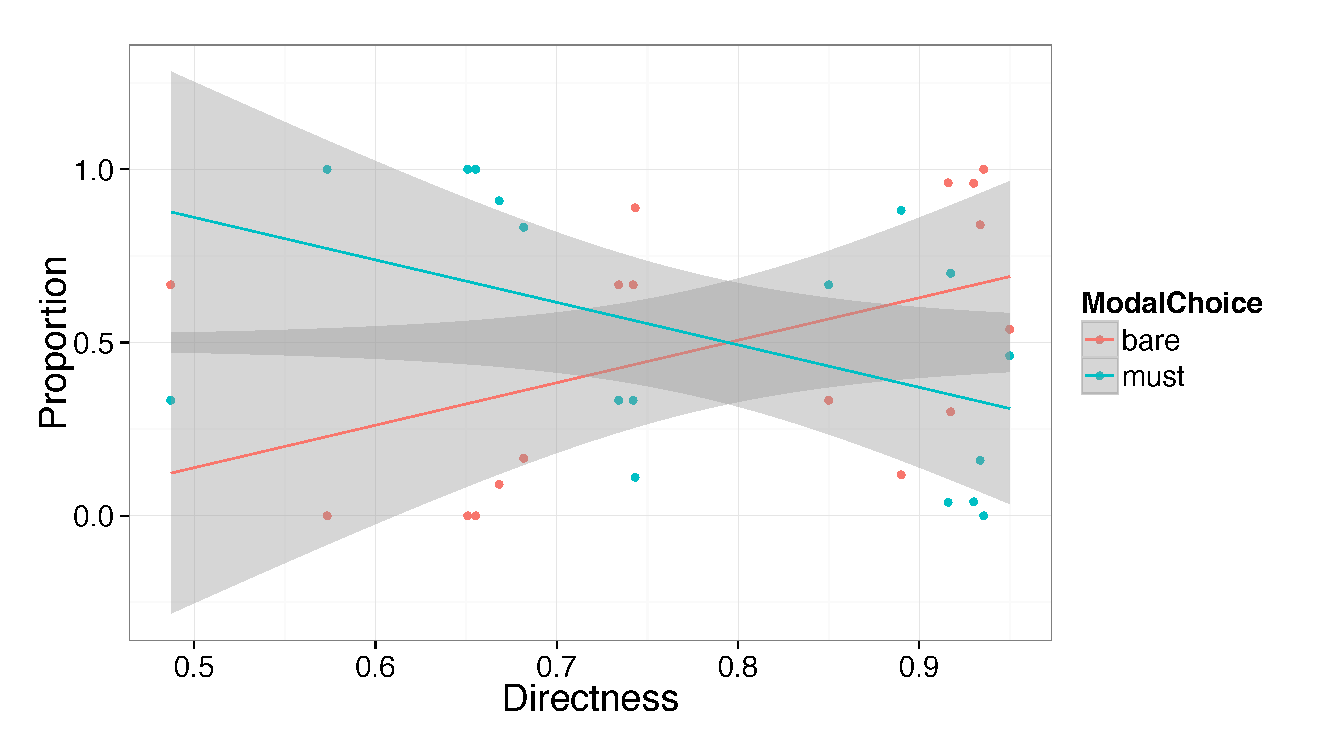
\includegraphics[width=\linewidth]{expt2.eps}}
%\caption{Utterance choice plotted against evidence strength (Expt.~2).}
%\label{expt2}
%\end{figure}


\section{Experiment E.3a: comprehension (listener belief)}

%Having found that speakers' use of \emph{must} increases as evidence strength decreases, we next tested whether listeners take into account this information about speakers as they interpret the bare and \emph{must} forms. In testing listeners' interpretation of \emph{must}, we also evaluated its relative strength.

We next tested the other side of the communicative coin: depending on the utterance $u$ used to communicate about $q$, how strong is listeners' resulting belief in $q$, and what do they believe to be the strength of the evidence the speaker was in possession of when producing $u$?\footnote{This experiment can be viewed \href{http://stanford.edu/~jdegen/72_modals_comprehension_evidence_room/modals.html}{here}.}

\subsection{Methods}

\subsubsection{Participants}

We recruited 120 participants through Amazon's Mechanical Turk. Participants were compensated with a small payment.

\subsubsection{Materials and procedure}

Participants were presented with an utterance (e.g., ``It must be raining'') and asked a) to rate the probability of the state of affairs \emph{q} (e.g., it is raining); and b) to select one out of five pieces of evidence that the speaker had about \emph{q} in making their utterance. On each trial, participants first saw two context sentences: ``You are in a windowless room. Your friend X walks in and says:'', where ``X'' was a randomly generated name.\footnote{This was done to discourage effects of inferences about speaker-specific language use on interpretation.} Participants then saw one of the utterances from Exp.~E.2 that ``X'' produced, e.g., ``It must be raining''. They were asked ``How likely do you think it is that it is raining?'' and adjusted a slider with endpoints labeled ``impossible'' and ``certain'' in response. Once they thus submitted their belief in $q$, the five potential pieces of evidence previously used in Exps.~E.1 and E.2 were shown and participants were asked to choose one by clicking a radio button in response to the question ``How do you think X knows about the rain?'' 

Participants provided one set of judgments for each domain, resulting in four trials per participant. Each participant saw each type of utterance (bare, must, probably, might)  across trials. Utterance types were randomly distributed across domains. Trial order was randomized, as was the order in which pieces of evidence were displayed.

\subsection{Results and discussion}

Fig.~\ref{fig:expt3a} shows mean probability of listener belief in $q$ by utterance: participants believed \emph{q} was less likely after observing the \emph{must} utterance than after observing the \emph{bare} utterance ($\beta$=-0.21, \emph{SE}=0.01, \emph{t}=-10.1, \emph{p}$<$0.0001). \figref{fig:evidencestrength-lbelief} shows mean evidence strength by utterance. \red{Analysis for both} %Fig.~\ref{expt3b} plots average strength of evidence assumed for each utterance. Average evidence strength was lower for \emph{must} than for the bare utterance ($\beta$=-0.08, \emph{SE}=0.01, \emph{t}=-6.8, \emph{p}$<$0.0001).

\begin{figure}
	\centering
	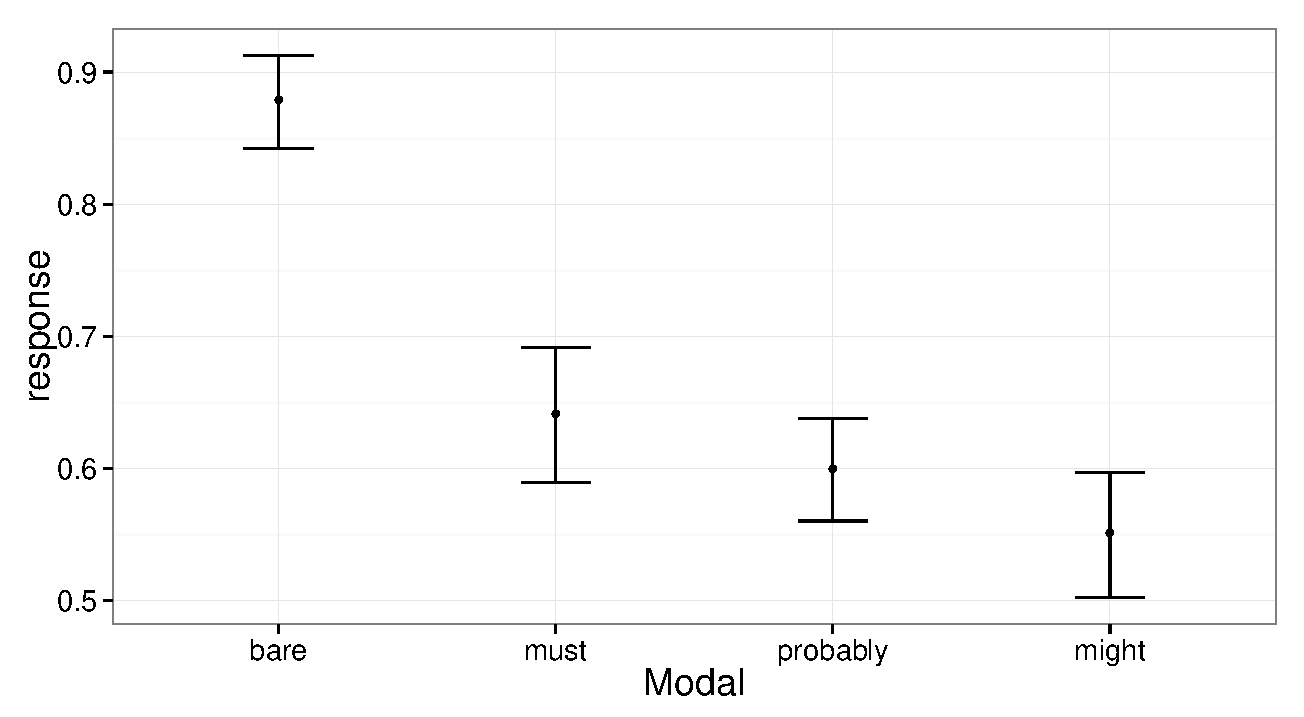
\includegraphics[width=\linewidth]{expt3a}
	\caption{\red{replace} Mean probability of listener belief in $q$ by utterance for English (left, Exp.~E.3a) and German (right, Exp.~G.3a). Error bars indicate 95\% bootstrapped confidence intervals.}
	\label{fig:expt3a}
\end{figure}

\begin{figure}
	\centering
%	\includegraphics[width=\linewidth]{expt3a-evidence}
	\caption{\red{replace} Mean inferred evidence strength by utterance for English (left, Exp.~E.3a) and German (right, Exp.~G.3a). Error bars indicate 95\% bootstrapped confidence intervals.}
	\label{fig:expt3a-evidence}
\end{figure}

\section{Experiment E.3b: comprehension (speaker commitment)}

%Having found that speakers' use of \emph{must} increases as evidence strength decreases, we next tested whether listeners take into account this information about speakers as they interpret the bare and \emph{must} forms. In testing listeners' interpretation of \emph{must}, we also evaluated its relative strength.

Exp.~3a tested listener beliefs in $q$ as a function of the observed utterance. A related, but potentially orthogonal dimension is the commitment that listeners ascribe to speakers as a basis for producing a particular utterance. For example, a particular utterance may lead the listener to infer that the speaker is highly committed to $q$, while nevertheless not instilling the same degree of belief in $q$ in the listener. In fact, epistemic \emph{must} has been claimed to function like this: vFG claim that maximal speaker commitment is necessary for the use of epistemic \emph{must}, just as in the use of the bare form; yet in comprehension the interpretation of \emph{must q} is weaker than that of bare $q$.  Exp.~E.3b thus tested the degree of belief in $q$ that listeners ascribe to \emph{speakers} depending on the utterance the speaker produced.\footnote{This experiment can be viewed \href{http://stanford.edu/~jdegen/80_modals_comprehension_speakerbelief/modals.html}{here}.}

\subsection{Methods}

\subsubsection{Participants}

We recruited 60 participants through Amazon's Mechanical Turk. Participants were compensated with a small payment.

\subsubsection{Materials and procedure}

The design, procedure, and materials were identical to those of Exp.~3a with the  exception of the dependent measure: instead of asking participants how likely they thought that $q$, they instead answered the question ``Does X think that it's raining?'' by adjusting a slider on a scale with endpoints labeled ``Definitely not'' and ``Definitely''. 

\subsection{Results and discussion}

Fig.~\ref{fig:expt3b} shows mean probability of speaker belief in $q$ (as ascribed by listeners) as a function of the speaker's utterance: \red{participants believed \emph{q} was less likely after observing the \emph{must} utterance than after observing the \emph{bare} utterance ($\beta$=-0.21, \emph{SE}=0.01, \emph{t}=-10.1, \emph{p}$<$0.0001). \figref{fig:evidencestrength-lbelief} shows mean evidence strength by utterance. }\red{Analysis for both} %Fig.~\ref{expt3b} plots average strength of evidence assumed for each utterance. Average evidence strength was lower for \emph{must} than for the bare utterance ($\beta$=-0.08, \emph{SE}=0.01, \emph{t}=-6.8, \emph{p}$<$0.0001).

\begin{figure}
	\centering
	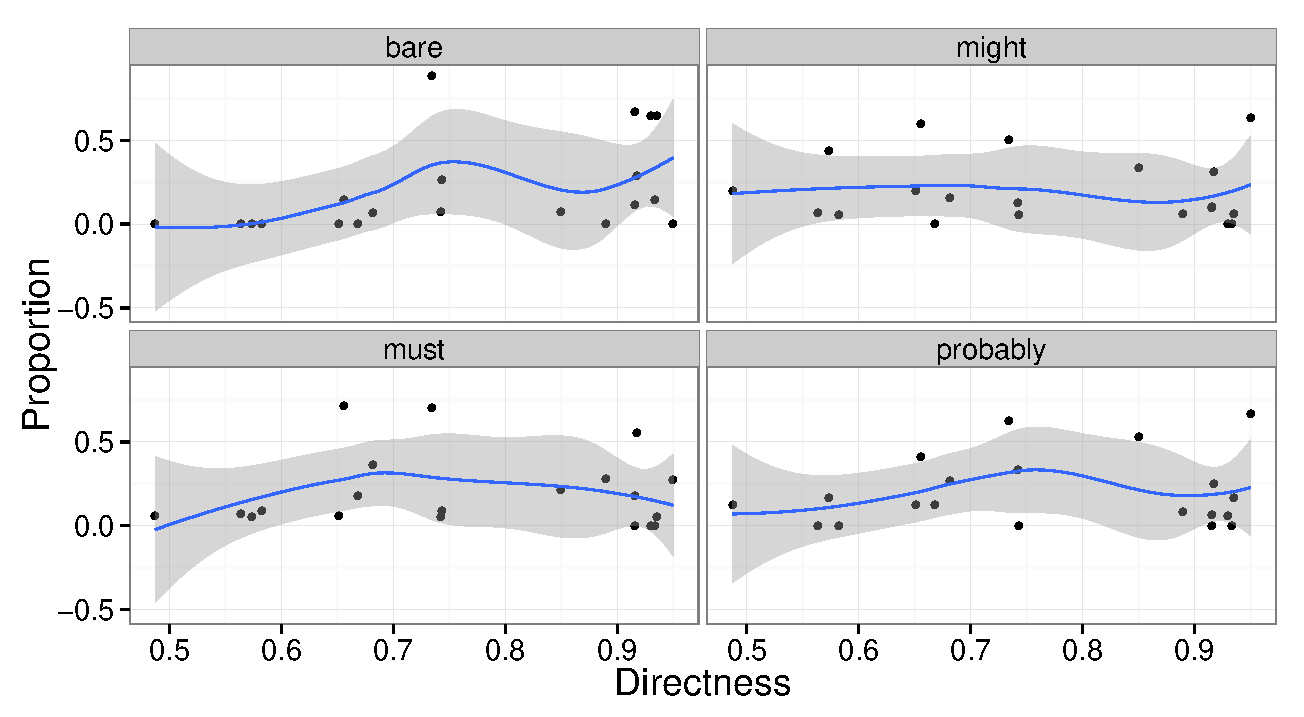
\includegraphics[width=\linewidth]{expt3b}
	\caption{\red{replace} Mean probability of ascribed speaker belief in $q$ by utterance for English (left, Exp.~E.3b) and German (right, Exp.~G.3b). Error bars indicate 95\% bootstrapped confidence intervals.}
	\label{fig:expt3b}
\end{figure}

\begin{figure}
	\centering
%	\includegraphics[width=\linewidth]{expt3b-evidence}
	\caption{\red{replace} Mean inferred evidence strength by utterance for English (left, Exp.~E.3b) and German (right, Exp.~G.3b). Error bars indicate 95\% bootstrapped confidence intervals.}
	\label{fig:expt3b-evidence}
\end{figure}

\section{Experiment G.1: evidence strength}

In this experiment we collected estimates of evidence strength for the same pieces of evidence as in E.1. The experiment was identical to E.1 with the exception that it was conducted in German. \footnote{This experiment can be viewed \href{http://web.stanford.edu/~jdegen/cgi-bin/4_dp_priors_evidencestrength/evidence.html}{here}.} 

\subsection{Methods}

\subsubsection{Participants}

\red{XXX} participants were recruited through Clickworker's crowd-sourcing service, and were compensated for their participation.

\subsubsection{Materials and procedure}

The procedure was identical to that of Exp.~E.1. All materials were translated into German. See \appref{sec:evidence} for the full list of stimuli.

\subsection{Results and discussion}

We obtained between \red{XX} and \red{XX} ratings for each piece of evidence. Participants' estimates of evidence strength are shown alongside those of the English-speaking participants in  \figref{fig:evidencestrength}. \red{diffs?} 

\section{Experiment G.2: production}

Next, we evaluated speakers' intuitions in a forced production task, testing how likely they are to use a particular form to communicate their belief about $q$ when given different pieces of evidence. The experiment was identical to E.2 with the exception that it was conducted in German and contained slightly different utterance choices.\footnote{This experiment can be viewed \href{http://web.stanford.edu/~jdegen/cgi-bin/3_dp_production/modals.html}{here}.}

\subsection{Methods}

\subsubsection{Participants}

We recruited \red{XXX} participants on the German crowd-sourcing service Clickworker. Participants were compensated with a small payment.

\subsubsection{Materials and procedure}

The procedure was identical to that of Exp.~E.2. As for participants' utterance choices, we included bare $q$ form and \emph{must q} as in Exp.~E.2, but instead of the modals \emph{probably} and \emph{might}, we included the modal adverbial \emph{vermutlich} (English \emph{presumably}) and the discourse particle \emph{wohl}. \red{issue of translating items into past perfect}

\subsection{Results and discussion}

Proportions of utterance choices for each piece of evidence are shown in \figref{fig:utterancesbyevidence} as a function of each piece of evidence's strength alongside the English results. In order to evaluate the effect of evidence strength on utterance choice, we conducted a mixed-effects model \red{looking at what exactly? multinomial regression?}. Of note are the following results: as evidence strength increases, the probability of producing the bare form increases (\red{XXX}). As evidence strength increases, the probability of producing \emph{must} \red{increases (XXX)}. As evidence strength increases, the probability of producing \emph{probably} \red{increases (XXX)}. And as evidence strength increases, the probability of producing \emph{might} \red{increases (XXX)}.

\section{Experiment G.3a: comprehension (listener belief)}

We next tested the other side of the communicative coin: depending on the utterance $u$ used to communicate about $q$, how strong is listeners' resulting belief in $q$, and what do they believe to be the strength of the evidence the speaker was in possession of when producing $u$? This experiment was identical to E.3a with the exception that it was conducted in German and included the slightly different set of utterance options used in Exp.~G.2.
\footnote{This experiment can be viewed \href{http://web.stanford.edu/~jdegen/cgi-bin/2_dp_comprehension_listenerbelief/modals.html}{here}.}

\subsection{Methods}

\subsubsection{Participants}

We recruited \red{XXX} participants through the German crowd-sourcing service Clickworker. Participants were compensated with a small payment.

\subsubsection{Materials and procedure}

The procedure was identical to that of Exp.~E.3a, but materials were presented in German and the utterances participants observed were the ones used in Exp.~G.2.

\subsection{Results and discussion}

Fig.~\ref{fig:expt3a} shows mean probability of listener belief in $q$ by utterance alongside the English results: as in English, participants believed \emph{q} was less likely after observing the \emph{must} utterance than after observing the \emph{bare} utterance ($\beta$=-0.21, \emph{SE}=0.01, \emph{t}=-10.1, \emph{p}$<$0.0001). \figref{fig:evidencestrength-lbelief} shows mean evidence strength by utterance. \red{Analysis for both} 

\section{Experiment G.3b: comprehension (speaker commitment)}

This experiment was a German version of Exp.~E.3b and tested the commitment that listeners ascribe to speakers after observing each of the four utterance types used in Exps.~G.2 and G.3a.\footnote{This experiment can be viewed \href{http://web.stanford.edu/~jdegen/cgi-bin/1_dp_comprehension_speakerbelief/discourse_particles.html}{here}.}

\subsection{Methods}

\subsubsection{Participants}

We recruited \red{XXX} participants through the German crowd-sourcing service Clickworker. Participants were compensated with a small payment.

\subsubsection{Materials and procedure}

The procedure was identical to that of Exp.~E.3b but was conducted in German and used the slightly different set of utterances.

\subsection{Results and discussion}

Fig.~\ref{fig:expt3b} shows mean probability of speaker belief in $q$ (as ascribed by listeners) as a function of the speaker's utterance alongside the English results: \red{participants believed \emph{q} was less likely after observing the \emph{must} utterance than after observing the \emph{bare} utterance ($\beta$=-0.21, \emph{SE}=0.01, \emph{t}=-10.1, \emph{p}$<$0.0001). \figref{fig:evidencestrength-lbelief} shows mean evidence strength by utterance. }\red{Analysis for both} 



\section{General discussion}

%\section{Model}

%We propose a computational model of language understanding to show that the empirically verified, relatively weak interpretation of \textit{must} does not require encoding weakness or indirectness into the semantics of modals, but can  arise instead from pragmatic reasoning about its strength. In fact, already in \citeA[pp.~33--34]{grice1989} do we find inspiration for the calculation that leads to the relative weakness of \emph{must}:
%
%\begin{quotation}
%	``A wants to know whether \emph{p}, and B volunteers not only the information that \emph{p}, but information to the effect that it is certain that \emph{p}\ldots\ B's volubility may be undesigned, and if it is so regarded by A it may raise in A's mind a doubt as to whether B is as certain as he says he is\ldots\ But if it is thought of as designed, it would be an oblique way of conveying that it is to some degree controversial whether or not \emph{p}.''
%\end{quotation}
%
%\noindent Here, we formalize \citeauthor{grice1989}'s description of the computation. 
%
%Our model follows the basic structure of Rational Speech Act (RSA) models, which view language understanding as recursive reasoning between speaker and listener \cite{frankgoodman2012}.

\section{Conclusion}


\appendix

\section{Pieces of evidence}
\label{sec:evidence}

This section lists, for each proposition $q$, the five pieces of evidence that were used throughout all experiments.

\subsection{It's raining. / Es hat geregnet.}

\begin{enumerate}
	\item You look out the window and see raindrops falling from the sky. \\ Sie sehen aus dem Fenster und beobachten, wie Regentropfen vom Himmel fallen. 
	\item You hear the sound of water dripping on the roof. \\ Sie k�nnen h�ren, wie Wasser auf das Dach prasselt.
	\item You check the weather report on the Internet, which says it is raining. \\ Sie haben im Internet den Wetterbericht gelesen, in dem stand, dass es regnen w�rde. 
	\item You see a person come in from outside with wet hair and wet clothes. \\ Sie sehen, wie jemand mit nassen Haaren und durchn�ssten Kleidern von drau�en hereinkommt.
	\item Earlier today, you had seen dark clouds in the sky. \\ Sie haben heute Vormittag dunkle Wolken am Himmel gesehen.
\end{enumerate}

\subsection{The coffee is cold. / Der Kaffee ist kalt geworden.}

\begin{enumerate} 
	\item You take a sip of the coffee and feel that it is cold. \\
	Sie trinken einen Schluck Kaffee und stellen fest, dass er kalt ist
	\item You touch the coffee cup and feel that it is cold.\\
	Sie ber�hren die Kaffeetasse und stellen fest, dass sie kalt ist.
	\item You see that there is no steam coming from the coffee.\\
	Sie sehen, dass aus dem Kaffee kein Dampf aufsteigt.
	\item You know that the coffee has been on the table for an hour.\\
	Sie wissen, dass der Kaffee seit einer Stunde auf dem Tisch steht.
	\item You see that the cup isn't insulated.\\
	Sie sehen, dass die Tasse nicht isoliert ist.
\end{enumerate}

\subsection{Dinner is ready. / Das Abendessen ist fertig geworden.}

\begin{enumerate}
	\item You just prepared dinner and set it out on the table.\\
	Sie haben gerade das Abendessen zubereitet und auf den Tisch gestellt
	\item Your spouse tells you that dinner is ready.\\
	Ihr/e Partner/in sagt, dass das Abendessen fertig ist.
	\item Dinner is usually ready at around 6pm. You look at the clock and it is 6pm.\\
	Sie wissen, dass das Abendessen normalerweise um 18 Uhr fertig ist. Ein Blick auf die Uhr zeigt, dass es gerade 18 Uhr ist.
	\item You smell food coming from the dining room.\\
	Sie vernehmen den Geruch von Essen, der aus dem Esszimmer kommt.
	\item You're hungry.\\
	Sie haben Hunger.
\end{enumerate}

\subsection{The neighbor's dog is barking. / Der Nachbarshund hat gebellt.}

\begin{enumerate}
	\item You look outside and see Fluffy, the neighbor's dog, standing on the porch and barking.\\
	Sie schauen aus dem Fenster und sehen Struppi, den Hund der Nachbarn, wie er am Zaun steht und bellt.
	\item You hear the sound of a dog barking.\\
	Sie h�ren einen Hund bellen.
	\item You are listening to music with your earphones. You know that your neighbor's dog often barks in the evening.\\
	Sie haben Kopfh�rer auf und h�ren Musik, wissen aber, dass der Hund der Nachbarn abends oft bellt.
	\item You are listening to music with your earphones. You look out the window and see that the mailman has just arrived at your neighbor's doorstep, when all of a sudden he jumps back.\\
	Sie haben Kopfh�rer auf und h�ren Musik, sehen aber aus dem Fenster und beobachten, wie der Postbote vor der Nachbarst�r einen Satz nach hinten macht.
	\item Your neighbor just got a new dog.\\
	Sie wissen, dass sich die Nachbarn gerade einen Hund angeschafft haben.
\end{enumerate}

\section{Acknowledgments}



\bibliographystyle{apacite}

\setlength{\bibleftmargin}{.125in}
\setlength{\bibindent}{-\bibleftmargin}

\bibliography{bibs}


\end{document}
